\documentclass[11pt]{article}
\usepackage[utf8]{inputenc}
\usepackage[T1]{fontenc}
\usepackage{amsmath}
\usepackage{amssymb}
\usepackage{graphicx}
\usepackage{geometry}
\usepackage{tikz}
\usepackage{ulem}
\usepackage{pgfplots}
% For underline, using normalem to avoid messing with \emph

\geometry{a4paper, margin=1in}
\usetikzlibrary{positioning, arrows.meta, shapes.geometric} % For TikZ diagrams

% Custom commands (optional)
\newcommand{\avg}[1]{\overline{#1}}
\newcommand{\prob}[1]{P(#1)}
\newcommand{\ProbDens}[1]{\mathcal{P}(#1)} % Using script P for density
\newcommand{\vect}[1]{\vec{#1}}
\newcommand{\dd}[1]{\mathrm{d}#1} % Differential d
\newcommand{\pderiv}[2]{\frac{\partial #1}{\partial #2}}
\newcommand{\deriv}[2]{\frac{\mathrm{d} #1}{\mathrm{d} #2}}
\newcommand{\qdot}{\dot{q}}
\newcommand{\pdot}{\dot{p}}
\newcommand{\muState}{\mu\text{-state}} % Microstate

\title{Physics 415 - Lecture 3: Statistical Description of Systems}
\date{January 27, 2025}
\author{} % Author not specified

\begin{document}

\maketitle
\thispagestyle{empty}

\section*{Statistical Description of System of Particles}

Use statistical ideas to go from microscopic ($\mu$-scopic) laws to macroscopic properties.

\begin{itemize}
    \item While the $\mu$-scopic world is governed by quantum mechanics (QM), it is often useful to consider the classical description (classical mechanics - CM) as well.
    \item We'll therefore go back \& forth between QM \& CM, starting now with CM.
\end{itemize}

\subsection*{Classical Mechanical Description}

Consider a mechanical system with $S$ degrees of freedom (DOF) associated with coordinates $(q_1, q_2, \dots, q_S)$ and momenta $(p_1, p_2, \dots, p_S)$.
\begin{itemize}
    \item \textbf{Example:} N particles in 3D. $S=3N$ DOFs. Coordinates $(\vec{x}_1, \vec{x}_2, \dots, \vec{x}_N)$.
    \item The state of the system at any time $t$ is completely determined by its $2S$ coordinates and momenta.
    \item The set $\{q_1(t), \dots, q_S(t), p_1(t), \dots, p_S(t)\}$ specifies the "microstate" ($\mu$-state) of the system.
    \item We need both $q$'s and $p$'s to specify the state because the equations of motion (EOM) of CM are second-order in time derivatives (like $\ddot{q}$) or first order for $q$ and $p$ (Hamilton's equations), requiring $2S$ initial conditions (e.g., $q_i(0)$ and $p_i(0)$ for all $i$).
\end{itemize}
Each $\mu$-state specifies a point in the $2S$-dimensional "phase space" of the mechanical system (coordinates $q_1, \dots, q_S, p_1, \dots, p_S$).

\textbf{Example:} For $S=1$ DOF, dimension of phase space = 2.

\begin{center}
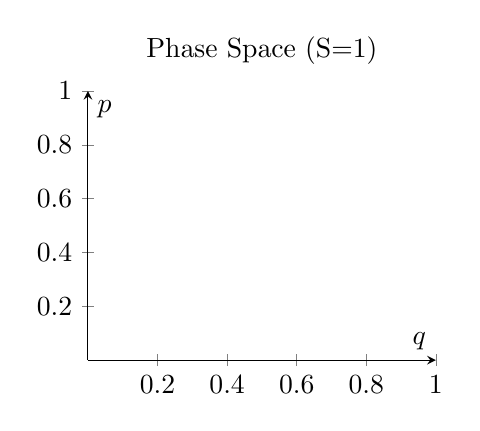
\begin{tikzpicture}
\begin{axis}[
    axis lines=middle, xlabel=$q$, ylabel=$p$,
    xtick=\empty, ytick=\empty,
    width=6cm, height=5cm,
    title={Phase Space (S=1)}
]
\coordinate (A) at (axis cs:1, 1.5);
\node at (A) [circle, fill=black, inner sep=1.5pt, label=above right:A] {};
\node at (axis cs: 1.8, 0.5) {A point in phase space};
\node at (axis cs: 1.8, 0) {specifies a $\mu$-state.};
\end{axis}
\end{tikzpicture}
\end{center}

A point A in phase space evolves according to "Hamilton's equations":
\begin{align*} \dot{q}_i &= \pderiv{H}{p_i} \\ \dot{p}_i &= -\pderiv{H}{q_i} \end{align*} 
for $i=1, \dots, S$.
\begin{itemize}
    \item $H(q,p)$ is the "Hamiltonian function".
    \item This is a system of $2S$ coupled first-order ODEs.
    \item $H(q,p)$ can usually be expressed as the energy of the mechanical system, written in terms of coordinates $q$ and momenta $p$.
\end{itemize}
The time evolution of $q_i(t)$ and $p_i(t)$ according to Hamilton's equations traces out an orbit (trajectory) in phase space.

\begin{center}
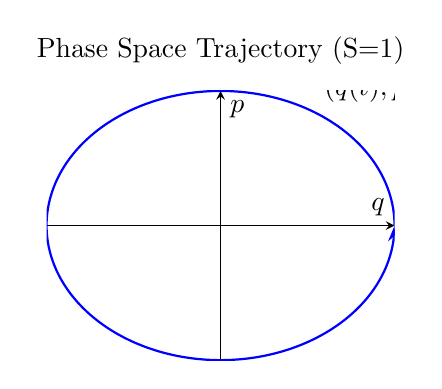
\begin{tikzpicture}
\begin{axis}[
    axis lines=middle, xlabel=$q$, ylabel=$p$,
    xtick=\empty, ytick=\empty,
    width=6cm, height=5cm,
    title={Phase Space Trajectory (S=1)}
]
% Example trajectory (e.g., ellipse for HO)
\addplot [domain=0:2*pi, samples=100, smooth, thick, blue, -{Stealth[length=2mm]}] ({cos(deg(x))}, {1.5*sin(deg(x))});
\node at (axis cs: {cos(deg(1))}, {1.5*sin(deg(1))}) [above right] {$(q(t), p(t))$};
\end{axis}
\end{tikzpicture}
\end{center}

\subsection*{Discretization of Phase Space}

In order to "count" all possible $\mu$-states, we conceptually discretize phase space into small cells.
\begin{itemize}
    \item For $S=1$ DOF: Divide phase space into cells of small "area" $\delta q \delta p = h_0$. A $\mu$-state is specified by a phase space cell.
    \item For $S$ DOF: Similarly, divide phase space into cells with "volume" $\delta q_1 \delta q_2 \dots \delta q_S \delta p_1 \delta p_2 \dots \delta p_S = h_0^S$. A $\mu$-state is again specified by a phase space cell. ($h_0$ has units of action, e.g., related to Planck's constant in QM link).
\end{itemize}


\subsection*{Statistical Approach}

Having specified the $\mu$-states in the classical case (the phase space cells), we now turn to the statistical approach of analyzing the many-particle system.

\textbf{Recall our motivation:} If we could specify all $2S$ initial conditions (say, for $N \sim 10^{23}$ particles $\implies S=3N \implies 2S \sim 6 \times 10^{23}$ conditions!) and time evolve Hamilton's equations, the state would be deterministic. However, this approach is neither practical nor useful. Instead, we seek statistical information regarding the macroscopic state of the system.

\section*{Statistical Ensemble}

To apply statistical/probabilistic concepts, we consider not a single isolated system, but rather an "ensemble" of a very large number $\mathcal{N} \gg 1$ of identical systems.
\begin{itemize}
    \item Each system in the ensemble is prepared under identical macroscopic conditions (e.g., same $N, V, E$).
    \item In general, systems in the ensemble will be in different $\mu$-states at any given time.
\end{itemize}

\begin{center}
\fbox{System 1 ($\mu$-state $\mu_1$, Pressure $P_1$)} \quad
\fbox{System 2 ($\mu$-state $\mu_2$, Pressure $P_2$)} \quad $\dots$ \quad
\fbox{System $\mathcal{N}$ ($\mu$-state $\mu_{\mathcal{N}}$, Pressure $P_{\mathcal{N}}$)}
\end{center}

Since each system is in a different $\mu$-state, each system (at a given time) will be characterized by potentially different values of macroscopic parameters that are not fixed (e.g., pressure $P$ might fluctuate if $E, V, N$ are fixed).
\textbf{Example:} Pressure of system 1 is $P_1$, pressure of system 2 is $P_2$, etc.

\textbf{Question:} What is the distribution of a macroscopic parameter (e.g., pressure) across the ensemble?

Before addressing this question, note that we can often place general constraints on the allowed $\mu$-states. For example, the total energy $E$, volume $V$, and number of particles $N$ may be fixed.
\begin{itemize}
    \item This means only those $\mu$-states compatible with these fixed values are allowed. These are the "accessible states".
\end{itemize}
To answer the question above, we need to know the probability $P(\mu_i)$ to find a system (chosen randomly from the ensemble at some time) in $\mu$-state $\mu_i$.

To make progress, we will assume the system is in "equilibrium".

\section*{Fundamental Postulate}

\begin{itemize}
    \item \textbf{Equilibrium} here means the probability $P(\mu_i)$ is independent of time. This implies all average macroscopic parameters are also time-independent.
    \item \textbf{Fundamental Postulate (Equal a Priori Probabilities):} An isolated system in equilibrium is equally likely to be in any of its accessible $\mu$-states.
    \item (Classical case: all accessible phase space cells are equally likely).
\end{itemize}

\textbf{Formulation:}
Consider an isolated system with volume $V$, consisting of $N$ particles, with fixed energy known to lie in some small range $(E, E+\delta E)$.
\begin{itemize}
    \item Let $\Omega(E)$ = total number of $\mu$-states (phase space cells) in this energy range.
    \item Then the probability $P(\mu_i)$ of finding the system in a particular accessible $\mu$-state $\mu_i$ is:
    \[ P(\mu_i) = \begin{cases} 1 / \Omega(E) & \text{if } \mu_i \text{ is accessible (Energy in range)} \\ 0 & \text{otherwise} \end{cases} \]
\end{itemize}

\textbf{Example:} 1D harmonic oscillator.
$H(q,p) = \frac{p^2}{2m} + \frac{1}{2} k q^2$.
$H(q,p) = E = \text{const}$ defines an ellipse in phase space.
States with energy between $E$ and $E+\delta E$ lie in the annular region between the ellipse for $E$ and the ellipse for $E+\delta E$.

\begin{center}
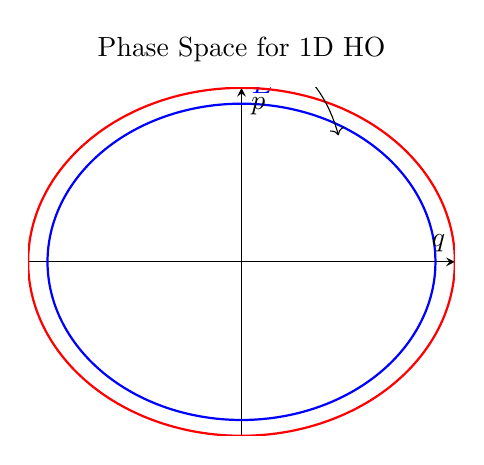
\begin{tikzpicture}
\begin{axis}[
    axis lines=middle, xlabel=$q$, ylabel=$p$,
    xtick=\empty, ytick=\empty,
    width=7cm, height=6cm,
    title={Phase Space for 1D HO}
]
% Ellipse for E
\addplot [domain=0:2*pi, samples=100, smooth, thick, blue] ({2*cos(deg(x))}, {1*sin(deg(x))}) node[pos=0.25, anchor=south west] {$E$};
% Ellipse for E + delta E
\addplot [domain=0:2*pi, samples=100, smooth, thick, red] ({2.2*cos(deg(x))}, {1.1*sin(deg(x))}) node[pos=0.25, anchor=south west] {$E+\delta E$};
% Indicate annular region (conceptual)
\node at (axis cs:0, 1.5) {Accessible states};
\draw [->, bend left] (axis cs:0, 1.4) to (axis cs:1, 0.8);
\end{axis}
\end{tikzpicture}
\end{center}
$$
\Omega(E) = \frac{\text{Area of annular region (between } E \text{ and } E+\delta E)}
{\text{Area of one phase space cell } h_0} = \text{Number of accessible states}
$$

\section*{Calculating Averages}

Using the fundamental postulate, we may now calculate probabilities and averages of interest.

Suppose we want to know the probability of the system having some particular value $y_k$ of a macroscopic parameter $Y$ (e.g., pressure $P=P_k$).
\begin{itemize}
    \item Let $\Omega(E; y_k) = \#$ of accessible states (energy in $(E, E+\delta E)$) for which the parameter $Y$ assumes the value $y_k$. (This is a subset of all $\Omega(E)$ accessible states).
    \item The probability of observing $Y=y_k$ is:
    \[ P(Y=y_k) = \frac{\text{\# states with } Y=y_k}{\text{Total \# accessible states}} = \frac{\Omega(E; y_k)}{\Omega(E)} \]
\end{itemize}
To find the mean (ensemble average) value of the parameter $Y$:
\[ \avg{Y} = \sum_k P(Y=y_k) y_k = \sum_k \frac{\Omega(E; y_k)}{\Omega(E)} y_k = \frac{1}{\Omega(E)} \sum_k \Omega(E; y_k) y_k \]

\end{document}